%%%%%%%%%%%%%%%%%%%%%%%%%%%%%%%%%%%%%%%%%%%%%%%%%
\section{Le corps des diapositives}

%++++++++++++++++++++++++++++++++++++++++++++++++
\subsection{Équations et formules}
%------------------------------------------------
\begin{frame}
	\frametitle{Suite d'équations avec \lin{align*}}
	\begin{align*}
		a 
		& = b+c+d * \sum_{i=1}^n x_i\\
		& = b+c+d * \sum_{i=1}^n (z_i - y_i)\\
		& \leqslant B+c+d * \sum_{i=1}^n (z_i - y_i) & 
		\textcolor{expli}{\textit{ ici une petite explication}}\\
	\end{align*}
\end{frame}

%------------------------------------------------
\begin{frame}
	\frametitle{Formules centrées, éventuellement encadrées\esp}
	Voilà une formule juste centrée car entre \lin{$$} et \lin{$$} 
	$$ A  = \sum_{i=1}^{n} a_i +b_i$$
	Voilà une formule encadrée avec \lin{\fbox} et centrée 
	\begin{center}
		\fbox{$\Delta^{early}_u\!(E,\!T) \!\geqslant 0$ if $u \in E$}
	\end{center}
	
	Voilà une formule encadrée en couleurs avec \lin{\fcolorbox} et centrée
	\begin{center}
		\fcolorbox{turquoiseFonce}{white}{$\Delta^{early}_u\!(E,\!T) \!\geqslant 0$ if $u \in E$}
	\end{center}
	NB: le deuxième argument de \lin{\fcolorbox} fixe la couleur du fond, je déconseille de l'utiliser avec une couleur franche, ainsi on évitera ça : 
	\fcolorbox{red}{blue}{$\Delta^{early}_u\!(E,\!T) \!\geqslant 0$ if $u \in E$} 
	et même
	\fcolorbox{green}{yellow}{$\Delta^{early}_u\!(E,\!T) \!\geqslant 0$ if $u \in E$} 
\end{frame}

%++++++++++++++++++++++++++++++++++++++++++++++++
\subsection{Environnements \lin{description} et \lin{minipage}}
%------------------------------------------------
\begin{frame}
  \frametitle{Exemples d'utilisation de l'environnement \lin{description}}
  On peut par exemple décrire le problème...
  \begin{description}
    \item[entrées:] première donnée\\
    deuxième donnée\\
    dernière donnée\\
    \item[sortie:] le résultat
  \end{description}
\end{frame}

%------------------------------------------------
\begin{frame}
  \frametitle{Exemples d'utilisation de l'environnement \lin{minipage}}
  
  \begin{minipage}{0.48\textwidth}
    Là, à gauche, une colonne qui fait presque la moitié de la slide, dans laquelle je peux écrire plein de choses et dont je peux constater la largeur complète grâce à 
    \lin{\hrule} \hrule
  \end{minipage}
  \hspace*{0.2cm}
  \begin{minipage}{0.48\textwidth}
    \hrule
    Là, à droite, une colonne qui fait presque la moitié de la slide, dans laquelle je peux écrire plein de choses et dont je peux constater la largeur grâce à \lin{\hrule}
    que j'ai mis cette fois en début de paragraphe
  \end{minipage}

  \vspace*{0.4cm}

  \begin{minipage}[t]{0.64\textwidth}
    NB: par défaut, l'alignement vertical des minipages est "centré", ce qu'on peut modifier avec l'option \lin{[t]}. 
    Ici on est entre \lin{\begin{minipage}[t]{0.64\textwidth}}
    et \lin{\end{minipage}}
  \end{minipage}
  \hspace*{0.2cm}
  \begin{minipage}[t]{0.32\textwidth}
    Ici une petite largeur donc peu de mots font vite une grande hauteur,
    Remarquez que bien que plus haute, le haut de cette mini-page est aligné avec celui de celle de gauche
  \end{minipage}
\end{frame}

%------------------------------------------------
\begin{frame}
  \frametitle{Attention avec \lin{minipage} sous beamer}
  
  \begin{minipage}{0.6\textwidth}
  	Comme on peut le voir ici, la somme des largeurs indiquées dans les minipage doit être moins que  \lin{\textwidth}, sans quoi la dernière minipage est renvoyée à la ligne comme on peut le voir ici où on a juxtaposé une \lin{{minipage}{0.6\textwidth}} et une \lin{{minipage}{0.4\textwidth}}.
  \end{minipage}
  \begin{minipage}{0.4\textwidth}
    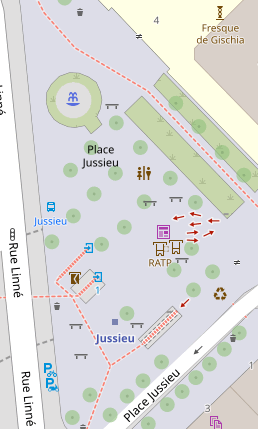
\includegraphics[scale=0.45]{pour_exemples/mini_plan.png}
  \end{minipage}
\end{frame}


%++++++++++++++++++++++++++++++++++++++++++++++++
\subsection{Minipages et inclusions (code, image)}
%------------------------------------------------
\begin{frame}
  \frametitle{Du texte et une image côte à côte}
  
  \begin{minipage}{0.56\textwidth}
    Lorem ipsum dolor sit amet, consectetuer adipiscing elit. 
    Ut purus elit, vestibulum ut, placerat ac, adipiscing vitae, felis. 
    Curabitur dictum gravida mauris. 
    Nam arcu libero, nonummy eget, consectetuer id, vulputate a, magna. 
    Donec vehicula augue eu neque. 
    Pellentesque habitant morbi tristique senectus et netus et malesuada fames ac turpis egestas. 
    Mauris ut leo. Cras viverra metus rhoncus sem. 
    Nulla et lectus vestibulum urna fringilla ultrices.
    Phasellus eu tellus sit amet tortor gravida placerat. Integer sapien est,
    iaculis in, pretium quis, viverra ac, nunc.
  \end{minipage}
  \hfill
  \begin{minipage}{0.38\textwidth}
    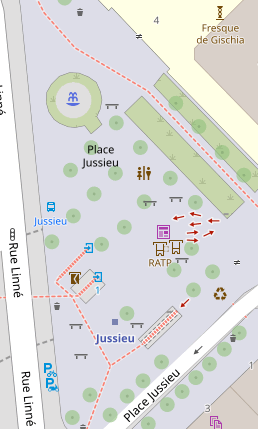
\includegraphics[scale=0.45]{pour_exemples/mini_plan.png}
  \end{minipage}
\end{frame}

%------------------------------------------------
\begin{frame}
  \frametitle{Du texte et du code C côte à côte\esp}
  
  \begin{minipage}{0.4\textwidth}
    Lorem ipsum dolor sit amet, consectetuer adipiscing elit. 
    Ut purus elit, vestibulum ut, placerat ac, adipiscing vitae, felis. 
    Curabitur dictum gravida mauris. 
    Nam arcu libero, nonummy eget, consectetuer id, vulputate a, magna. 
    Donec vehicula augue eu neque. 
  \end{minipage}
  \begin{minipage}{0.58\textwidth}
    \inputminted[firstline=3, lastline=8,firstnumber=1]{c}{pour_exemples/main.c}
  \end{minipage}
\end{frame}

%------------------------------------------------
\begin{frame}
  \frametitle{Une image et du code Ocaml côte à côte\esp}
  
  \begin{minipage}{0.28\textwidth}
    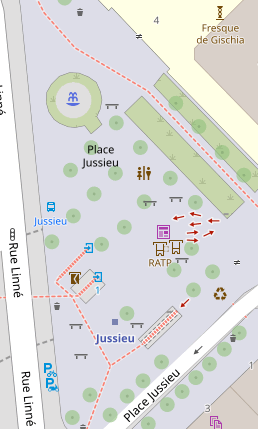
\includegraphics[scale=0.35]{pour_exemples/mini_plan.png}
  \end{minipage}
  \begin{minipage}{0.68\textwidth}
    \inputminted[firstline=1, lastline=10,firstnumber=1]{ocaml}{pour_exemples/test.ml}
  \end{minipage}
\end{frame}

%------------------------------------------------
\begin{frame}
  \frametitle{Deux images côte à côte}

  \begin{minipage}{0.49\textwidth}
	  \begin{figure}
		  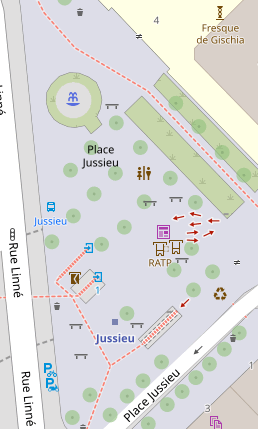
\includegraphics[scale=0.35]{pour_exemples/mini_plan.png}
		  \caption*{Une première image : un plan}
	  \end{figure}
  \end{minipage}
  \hfill
  \begin{minipage}{0.49\textwidth}
    \begin{figure}
		  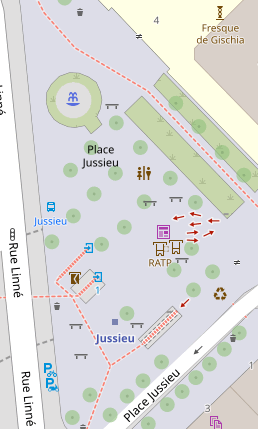
\includegraphics[scale=0.35]{pour_exemples/mini_plan.png}
		  \caption*{Une deuxième image : la même}
	  \end{figure}
  \end{minipage}
\end{frame}

%++++++++++++++++++++++++++++++++++++++++++++++++
\subsection{Une diapositive avec du pseudo-code}
%------------------------------------------------
\begin{frame}
	\small
	\frametitle{Pseudo-code avec \lin{algorithm} du package \lin{algo2e}}
	\begin{algorithm}[H]
		\caption{\textsf{Dijkstra}}
		\Input{Un graphe pondéré $G = (S, A,c)$ où $c : A \rightarrow \mathbb{R}^{+}$, $s\!\in\! S$}
		\Output{La distance de $s$ à chaque sommet de $S$}
		\BlankLine
		Initialiser $\delta[u]$ à $+\infty$ pour $u \in S$\;
 		Initialiser $\pi[u]$ à $\textsf{??}$ pour $u \in S$\;
  		$\delta[s] \gets 0$\;
  		%{\footnotesize\tcc*{~La source est à distance 0 d'elle-même }}	
 		$\pi[s] \gets s$\;
 		%{\footnotesize\tcc*{~La source est la racine de l’arborescence }}
  		$\textsf{todo} \gets \{s\}$\;
  		%{\footnotesize\tcc*{~La racine est le premier sommet à traiter }}
  		\Tq{$\textsf{todo} \neq \emptyset$}{
   			 Soit $u \in \textsf{todo}$ minimisant $\delta[u]$\;
    			\ForEach{$v \in \textsf{voisin}(u)$}{ 
    				$\textsf{Relacher}(G, u, v ,\delta, \pi, \textsf{todo})$
   			}
    			Ôter $u$ de $\textsf{todo}$ \;
  		}	
 	\Return{$\delta$}
\end{algorithm}
\end{frame}

%++++++++++++++++++++++++++++++++++++++++++++++++
\subsection{Astuces pour s'étaler en largeur}
%------------------------------------------------
\begin{frame}
  \frametitle{Moins de marge (ou plus?)}

  \begin{adjustwidth}{-1.5 em}{-1.5em}
    Ce paragraphe est entre 
    \lin{\begin{adjustwidth}{-1.5 em}{-1.5em}} et \lin{\end{adjustwidth}}
    ce qui lui permet de s'étaler  d'un bout à l'autre de la slide.
    En fait on a réduit les marges à gauche et à droite de 1.5em,
    on peut aussi augmenter les marges (réduire la largeur du texte donc) en mettant des valeurs positives, cf paragraphe juste après
  \end{adjustwidth}
  
  \bigskip
  
  \begin{adjustwidth}{2 em}{5em}
    Ce paragraphe est entre 
    \lin{\begin{adjustwidth}{2 em}{5em}} et \lin{\end{adjustwidth}}
    ce qui lui permet de s'étaler sur une largeur plus petite,et décalée vers la gauche.
    En fait on a augmenté la marge à gauche de 2em, et celle à droite de 5em
  \end{adjustwidth}
\end{frame}




